% $Author: ducasse $
% $Date: 2005/05/16 13:38:15 $
% $Revision: 1.1.1.1 $

\ifx\wholebook\relax\else
\documentclass{report}
\usepackage{times}
\usepackage{epsfig}
\usepackage{alltt}
\usepackage{xspace}
\usepackage{graphicx}
\usepackage{ifpdf}
\usepackage{ifthen}
\usepackage{amsmath}
\usepackage{a4wide}

\graphicspath{{figures/}} 

\ifpdf
\DeclareGraphicsExtensions{.pdf, .jpg, .tif, .png}
\else
\DeclareGraphicsExtensions{.eps, .jpg}
\fi

\newboolean{toseecomment}
\setboolean{toseecomment}{false}
%%change to false to hidde comment 
\newcommand{\comment}[1]{\ifthenelse{\boolean{toseecomment}}{$\blacktriangleright$ \textit{#1}$\blacktriangleleft$}{}}

\newcommand{\commented}[1]{}

\newboolean{seevwspecific}
\setboolean{seevwspecific}{true}
\newcommand{\vwspecific}[1]{\ifthenelse{\boolean{seevwspecific}}{#1}{}}

\newboolean{seecategoryspecific}
\setboolean{seecategoryspecific}{false}
\newcommand{\categoryspecific}[1]{\ifthenelse{\boolean{seecategoryspecific}}{#1}{}}

\newboolean{seestorespecific}
\setboolean{seestorespecific}{true}
\newcommand{\storespecific}[1]{\ifthenelse{\boolean{seestorespecific}}{#1}{}}

\newboolean{seesqueakspecific}
\setboolean{seesqueakspecific}{false}
\newcommand{\squeakspecific}[1]{\ifthenelse{\boolean{seesqueakspecific}}{#1}{}}


\newcommand{\category}[0]
{\ifthenelse{\boolean{seestorespecific}}
	{package\xspace}
	{category\xspace}}

\newcommand{\ct}[1]{\texttt{#1}\xspace}
\newcommand{\stc}[1]{{\small {\sf #1}}\xspace}
\newcommand{\ST}{{\textsc Smalltalk}\xspace}
\newcommand{\tab}{\makebox[4em]{}}
\newcommand{\ttt}[1]{{\tt #1}}
\newcommand{\chev}{\ttt{>>}}
\newcommand{\vw}{VisualWorks\xspace}
\newcommand{\sq}{Squeak\xspace}
\newcommand{\store}{Store\xspace}
\renewcommand{\chaptername}{Exercise}
\newcommand{\exercise}{\vspace{0.2cm}\noindent \textbf{Exercise:}\xspace}

\newsavebox{\fminibox}
\newlength{\fminilength}

% Fait un truc encadre
\newenvironment{fminipage}[1][\linewidth]
  {\setlength{\fminilength}{#1-2\fboxsep-2\fboxrule}
        \begin{lrbox}{\fminibox}\begin{minipage}{\fminilength}}
  { \end{minipage}\end{lrbox}\noindent\fbox{\usebox{\fminibox}}}

% Pareil mais pas encadre (a utiliser pour ne pas couper une fonction

\newenvironment{nminipage}[1][\linewidth]
  {\setlength{\fminilength}{#1}
        \begin{lrbox}{\fminibox}\begin{minipage}{\fminilength}}
  { \end{minipage}\end{lrbox}\noindent\mbox{\usebox{\fminibox}}}

% Un alltt encadre
\newenvironment{falltt}
  {\vspace*{0.3cm}\begin{fminipage}\begin{alltt}}
  {\end{alltt}\end{fminipage}\vspace*{0.3cm}}

% Un alltt pas encadre
\newenvironment{nalltt}
  {\vspace*{0.3cm}\begin{nminipage}\begin{alltt}}
  {\end{alltt}\end{nminipage}\vspace*{0.3cm}}

% Une fonction encadree
\newenvironment{ffonction}[1]
  {\begin{fonction}[#1]
        \begin{fminipage}
\begin{alltt}
\rule{\linewidth}{0.5pt}}
{\end{alltt}\end{fminipage}\end{fonction}}

\newenvironment{codeonepage}
  {\begin{nminipage}\vspace*{0.2cm}\hrule\vspace*{0.1cm}
\begin{alltt}}
  {\end{alltt} \vspace*{-0.2cm}\hrule \vspace*{0.2cm} \end{nminipage}}

\newenvironment{code}
  {\vspace*{0.1cm}\hrule\vspace*{-0.1cm}\begin{alltt}}
  {\end{alltt}\vspace*{-0.2cm}\hrule \vspace*{0.1cm}}


\begin{document}
\fi

\chapter{Building an Interface in VW}

In this lesson you will define a user interface for your application in \VW.


\mainauthor{Wuyts}
\sd{Rescue what roel wrote in word long time ago. and also provide the screenshots}


\section{ApplicationModel: the Glue between Domain and Widgets}

The class \ct{ApplicationModel} already: 
\begin{itemize}
\item defines basic application behavior (opening, running, closing, minimizing, �)
\item can open an application interface. 
\end{itemize}

Our application subclass will have to implement
\begin{itemize}
\item the actual interface to be opened,
\item behavior specific for your application,
\item glue code, to glue together the models and View/Controllers.
\end{itemize}

Basically, our application class will thus implement application specific code, 
thereby linking the views/controllers used in the interface with the domain
model. As explained in the lecture, models and view/controllers do not know 
each other directly, but will each talk to the applicationModel that actually 
glues everything together.

Building an application (\ie constructing a subclass of \ct{ApplicationModel}) 
thus boils down to two steps:
\begin{itemize}
\item building the interface
\item programming the applicationModel
\end{itemize}

\section{Building the interface}
Now we will need to build the interface as pictured above. 
An interface contains several widgets (user interface elements), 
in this case an input field and two buttons. There are several kinds of widgets:

\begin{itemize}
\item data widgets (gather/display input): let the user enter information, or display information
\item action widgets (invoke operations): buttons or menus, e.g. to increment or decrement the counter
\item static widgets (organise/structure the interface): labels identifying other widgets for the user.
\end{itemize}

You build an interface by creating a visual specification of the 
contents and the layout. To do so, there are several steps to be 
taken:
\begin{enumerate}
\item opening a blank canvas,
\item painting the canvas with widgets chosen from a Palette,
\item setting properties for each widget and applying them to the canvas,
\item installing the canvas in an application model.
\end{enumerate}

\paragraph{Step 1: opening a blank canvas}

\begin{figure}[htbp]
\begin{center}
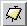
\includegraphics{nlesson11Fig2}
\caption{to do}
\end{center}
\end{figure}


A canvas is the place where you visually edit the interface of the application.
To open a blank canvas,  use the canvas button (as shown above) on the
VisualWorks Launcher, or select New Canvas in the Tools menu of the VisualWorks 
Launcher. VisualWorks will open a window containing an unlabeled canvas, 
a Canvas Tool, and a palette:
\begin{itemize}
\item the canvas tool provides you with the basic operations to build/install/define and open your application.
\item the palette contains predefined widgets to use on the canvas.
\item the unlabeled canvas is a visual representation for the window we are going to build. 
\end{itemize}


\paragraph{Step 2: painting the canvas}
We will now paint the widgets such that our interface looks l
ike the one pictured above. Basically this comes down on 
selecting widgets on the palette (by clicking them once), 
and putting them on the canvas (by clicking once again). 


\begin{figure}[htbp]
\begin{center}
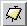
\includegraphics{nlesson11Fig2}
\caption{to do}
\end{center}
\end{figure}

 
 

First, we will put an input field on our canvas. To do so, follow these steps:
\begin{enumerate}
\item   verify that the single-selection button on the palette is active (it should look like the picture above). This enables you to paint a single copy of a widget on the canvas.
\item   note that, when you select a widget on the palette, the name of the selected widget is shown in the indicator field at the bottom of the palette.
\item   select the Input Field widget  by clicking it once (if you select the wrong widget, select other widgets until the indicator field displays Input Field).
\item   paint the input field by moving the mouse pointer to the canvas and clicking the select button once, positioning the widget, and clicking the select button a second time to place it on the canvas. 
\end{enumerate}

Once widgets are painted on the canvas, there are several editing operations that can be performed:
\begin{enumerate}
\item   to select a widget: click it once
\item   to deselect a widget: hold down the shift button while clicking on the selected widget, or click somewhere outside the widget
\item   to resize a widget: select the widget, click on one of the handles of the widget (the black squares at the outside of the widget) and resize it.
\item   to move a widget: select it, press the select button between the handles of the widget and move it
\item   to cut/copy a widget: select the widget, bring up the operate menu and select cut/copy in the edit menu
\item   to paste a widget (once you have cut/copied it): bring up the operate menu anywhere on a canvas, and select paste from the edit menu. The pasted widget is automatically placed at the same position as the widget that is cut/copied, and is automatically selected. You can now move it to another position.
\end{enumerate}


\exercise  copy the one button widget that is currently on the canvas to make a second one, and position the two buttons according to the picture of the application.


\paragraph{Step 3: setting and applying properties of widgets}
We now have painted widgets, and are ready to set their properties. 
Properties define a variety of visual attributes, the nature of the data they 
use or display, and how that data is referenced by the application. We will now
specify the different properties for our input field and buttons. 

To display a widget�s properties, we use the so-called Properties Tool. To open 
this tool, select the input field and click the Properties button on the Canvas
Tool. The properties tool opens, and we are now ready to examine and change the 
properties that are available for an input field. 

The properties are always arranged in a notebook, containing several pages. 
By clicking a tab of such a page, you select that page. Note that a Properties 
Tool does not belong to a particular canvas, or a particular widget.
For example, if you now select one of the two buttons, the Properties 
Tool will change to allow you to view/change the properties for that widget.

We will now fill in the properties for the input field. Select the input
field widget on the canvas. Go to the Basics page. Type in the aspect field:
counterValue (always start aspect names with a small letter), and select Number
in the type box. Apply these changes to the widget by pressing the apply button.
You can now select the Details page. On this page, mark the check box Read-Only.
Also apply these changes too. 

Just to be a little bit less blind. The symbol that you typed in the aspect
field corresponds to the selector of a method that we will create after. 
This method will return the model corresponding to the input field. 
Here as you will see the model will be value holder on the Number. 
This means that the valueHolder on a number will be the model (of the 
MVC pattern) for the inputField widget. The model of the InputField 
will be a ValueHolder, a basic object that send the message update to 
its dependent when it receives the message value:. 

\exercise: Set and apply the following properties for the left button:

Page    Property        Setting
Basics  Label   increment
        Action  increment
        Be Default      checked
The symbol associated with the Action button is the selector of a method of the application model that will be invoked when the button is pressed. 
Exercise: Set and apply these properties for the right button:
Page    Property        Setting
Basics  Label   decrement
        Action  decrement
        Be Default      unchecked
        Size as Default unchecked
        
        
\paragraph{Step 4 : Installing the canvas on an application model}
At any time in the painting process, you can save the canvas by 
installing it in an application model. Installing a canvas creates an 
interface specification, which serves as the application�s blueprint 
for building an operational window. An interface specification is a 
description of an interface. Each installed interface specification 
is stored in (and returned by) a unique class method in the application 
model by default named \ct{windowSpec}. Note that a same interface specification
can be save with different names, more interesting a same set of widget
can be saved in different positions under different method name. 

You can think of a canvas as the VisualWorks graphical user interface for creating and editing an interface  specification. Whereas a canvas is a graphical depiction of the window�s contents and layout, an interface specification is a symbolic representation that an application model can interpret.

To install a canvas:
\begin{itemize}
\item   click Install... in the canvas tool
\item   a dialog box comes up where you have to provide the name of the application model and the class method in which to install the canvas. Provide SimpleCounterApp as class name. Leave windowSpec (the default name of the class method where the interface specification is stored) as name of the selector. Press OK when finished.
\item   since your application model does not exist yet, you get another dialog box where you have to provide some information concerning your application model. Leave the name of the class, but provide \ct{DemoCounter} as name for the category. Since we are creating a normal application (and not a dialog box or so), choose the application check box. Note that VisualWorks then fills in \ct{ApplicationModel} as superclass. Leave this and select OK. Select a second time OK to close the first dialog box. 
\end{itemize}


The canvas is now installed on the class SimpleCounterApp. Open a browser, 
go to the category DemoCounter, select the class switch to see the class 
methods, and note that there is a method windowSpec in a protocol called 
�interface specs�. 

\section{Programming the application model}
As said in previous section, we now have to program our application model to:
specify the interface�s appearance and basic behavior,
supplement the application�s basic behavior with application-specific behavior.

As said before there are several kinds of widgets: static widgets,
action widgets and data widgets. Each of these kinds of widgets needs 
special programming care.

\paragraph{Static Widgets}
These are widgets like labels and separators that have no controller since they are just used to display something, and do not accept any kind of user input. No programming is required in the application model for this kind of widgets.

\paragraph{Action Widgets}

An action widget delegates an action to the application model from which it was built. Thus, when a user activates an action widget (for example, clicking the increment button), a message is sent by the widget to our application model (an instance of the class \ct{SimpleCounterApp}). What message is sent is defined in the properties of the widget, in the Action field on the Basics page. Since we have defined the action property of the left button to be increment, this means that a message increment is sent to the application model when the user presses the increment button. 

\paragraph{Data Widgets}
A data widget is designed to use an auxiliary object called a value model 
to manage the data it presents. (The value model play the M of the MVC pattern. 
This means that it propagates an update message to its dependent, the widget.) 
Thus, instead of holding on to the data directly it delegates this task to a 
value model:

\begin{itemize}
\item when a data widget accepts input from a user, it sends this input to its value model for storage,
\item when a data widget needs to update its display, it asks its value model for the data to be displayed.
\end{itemize}

The basic way to set up this interaction between a widget and its value 
model is by:
\begin{itemize}
\item   telling a widget the name of its value model (in our input field 
we filled in the aspect field on the basics page with counterValue, telling
the widget to use a message with this name to access  its value model in 
the application model.
\item   programming the application model such that it is able to create
and return this value model. For example, since we have provided counterValue 
as name for of the message that will be used by the input field widget to 
access its valueModel, we will have to provide this message in the class 
\ct{SimpleCounterApp}.
\end{itemize}

\paragraph{Defining stub methods, and opening the application}
As was said in the beginning, the application model is the glue for the 
models and the views/controllers. This means we have to implement:

\begin{itemize}
\item   methods for every data widget to let the widget access its value model,
\item   methods that perform a certain action and that are 
triggered by action widget.
\end{itemize}

Luckily, VisualWorks helps us with this step by generating stub-methods, methods with a default implementation that can then be changed to provide the desired behavior. To create such methods, we have to fill in the properties for every widget on our canvas (which we have done in previous steps), and then we use the define property.

\paragraph{To define properties:} deselect every widget on the canvas, 
and select the define button on the canvas tool. A list will come up with 
all the models where the system will create stub methods for. Leave all 
the models selected and press OK. The system will now generate the stub 
methods.

Note that often it is better to write by yourself the code generated, 
because you can have the control of the way the value model are created 
and accessed. 

We now have a basic application that we can open. To do so, select the 
Open button on the canvas tool.. You now can click on the buttons, but 
since we have not yet provided any actions, the default action happens 
(which is to do nothing). 

Go to your browser again, and deselect the class \ct{SimpleCounterApp}, and 
select it again. Set the switch to instance, and you will notice that 
the generation process added some methods:
\begin{itemize}
\item two methods in the action protocol: increment and decrement,
\item a method counterValue in a protocol aspects.
\end{itemize}

\section{About value models}
In previous section we explained that a data widget holds on to a 
value model, and that this value model actually holds the model. 
A data widget performs two basic operations with its value model:
\begin{itemize}
\item ask the contents of the value model using the value message, 
\item set contents of the value model using the value: message.
\end{itemize}

VisualWorks provides a whole hierarchy of different value models in the 
class \ct{ValueModel} and its subclasses. The simplest is \ct{ValueHolder}: it wraps 
any kind of object, and allows to access it using \ct{value} (to get the stored 
object) and \ct{value:} (to set the object). Sending the message \ct{asValue} to that 
object creates a valueholder on an object. Moreover using a valueHolder ensure
that its dependents receive the message \ct{update:}, each time the value model 
receives \ct{value:}.

In our application, we have an input field that should display a number. 
The input field is a data widget, so it has to hold on to a value model. 
This value model will actually store a number.  Note that the 
Model-View-Controller principle tells us that the data widget 
(a view-controller pair) should not know its model directly. 
Therefore, the input field only knows that it has to send counterValue 
to the application model, and the model knows nothing (since it is wrapped
in a value model). This means that we have to program our application model
so that it provides the correct  mapping.

If  you look at the implementation of the method counterValue 
(a stub method generated by the define command), you will see 
the following piece of code:

\begin{scode}
SimpleCounter\sep{}counterValue
        "This method was generated by UIDefiner.  Any edits made here
        may be lost whenever methods are automatically defined.  The
        initialization provided below may have been preempted by an
        initialize method."

        ^counterValue isNil
                ifTrue: [ counterValue := 0 asValue ]
                ifFalse: [ counterValue ] 
\end{scode}

This code implement a lazzy initialization of the value model. This means that if the valueModel (\ct{counterValue}) is defined, it is created, stored and return. If the valueModel is already defined, it is just simply return. Note that this is the method that is sent by the input field to access its value model.

Note such kind of lazzy initialization can be replaced by the following methods:

\begin{scode}
SimpleCounter\sep{}initialize
        super initialize.
        counterValue := 0 asValue.

SimplieCounter\sep{}counterValue
        ^ counterValue
\end{scode}

The following code only works that the initialize method is automatically invoke when the application model is created. This is the case because the class ApplicationModel class defines a class method new as follows.

\begin{code}
ApplicationModel\sep{}new
        ^super new initialize
\end{code}

\exercise Provide the implementation for increment and decrement, and test it.


\ifx\wholebook\relax\else\end{document}\fi